\documentclass[sigconf,authorversion]{acmart}
\acmDOI{}

% -- basic config
\usepackage{array} % support p{width}
\usepackage{tabularx} % flexible column X
\usepackage{booktabs} % \toprule, \midrule, \bottomrule
\usepackage{listings} % code listing
\usepackage{subcaption} % subfigures
\usepackage{ragged2e} % \justify
\usepackage{graphicx} % includegraphics
\usepackage{acronym} % \newacro and \ac
\usepackage{lipsum}
\usepackage{url} % \url
\newcommand{\ie}[0]{\textit{i.e.},~}
\newcommand{\eg}[0]{\textit{e.g.},~}
\newcommand{\etal}[0]{\textit{et al.}~}

% -- basic tikz
\usepackage{tikz}
\usetikzlibrary{arrows.meta, positioning, shapes, fit}

%%%%%%%%%%%%%%%%%%%%
\begin{document}
%%%%%%%%%%%%%%%%%%%%

\title{Title}
\author{Alan L. V. Guedes}
\email{a.guedes@reading.ac.uk}
\orcid{0000-0003-0110-9975}
\affiliation{%
    \institution{University of Reading}
    \city{Reading}
    \country{UK}
}
\renewcommand{\shortauthors}{Guedes, A.L.G.}

\begin{abstract}
\lipsum[1]
\end{abstract}
\keywords{keyword1, keyword2}

\maketitle

%%%%%%%%%%%%%%%%%%%%
\section{Introduction}
\label{sec:introduction}
%%%%%%%%%%%%%%%%%%%%

\begin{figure}[ht!]
\centering
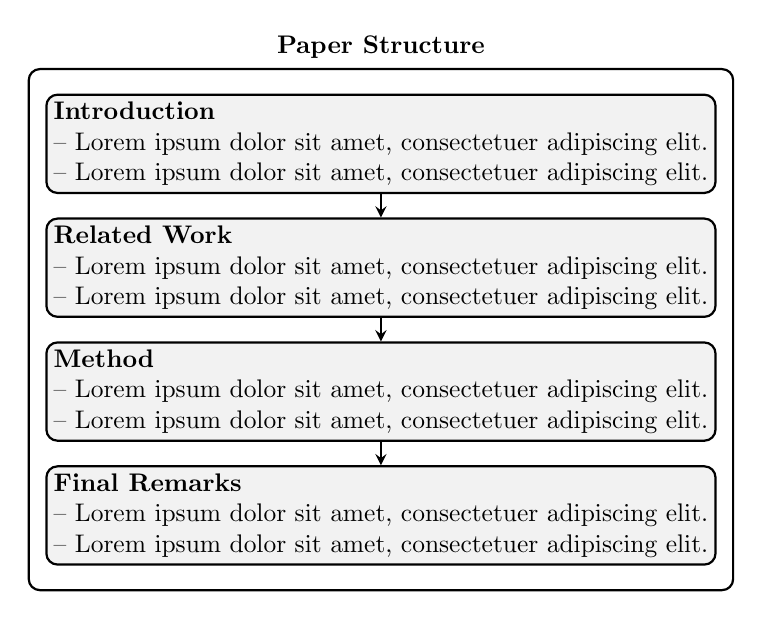
\begin{tikzpicture}[node distance=3mm,>=stealth,thick,scale=0.92, every node/.style={scale=0.92}]
  \tikzstyle{stage}=[rectangle, rounded corners, draw, align=flush left, minimum width=0.3\linewidth, inner sep=1mm]
  % Workflow nodes
  \node[stage, fill=gray!10] (pre) {\textbf{Introduction}\\
    -- \lipsum[1][1]\\
    -- \lipsum[1][1]
  };
  \node[stage, fill=gray!10, below=of pre] (prod) {\textbf{Related Work}\\
    -- \lipsum[1][1]\\
    -- \lipsum[1][1]
  };
  \node[stage, fill=gray!10, below=of prod] (post) {\textbf{Method}\\
    -- \lipsum[1][1]\\
    -- \lipsum[1][1]
  };
  \node[stage, fill=gray!10, below=of post] (dist) {\textbf{Final Remarks}\\
    -- \lipsum[1][1]\\
    -- \lipsum[1][1]
  };
  % Arrows between stages
  \draw[->] (pre.south) -- (prod.north);
  \draw[->] (prod.south) -- (post.north);
  \draw[->] (post.south) -- (dist.north);
  % Big surrounding box
  \node[draw, thick, rounded corners, fit=(pre)(prod)(post)(dist), inner sep=6mm, label={\textbf{Paper Structure}}] {};
\end{tikzpicture}
\caption{Structure.}
\Description{}
\label{fig:structure}
\end{figure}

\lipsum[1]\cite{TeXFAQ}, \cite{Downes04:amsart}

%%%%%%%%%%%%%%%%%%%%
\section{Related Work}
\label{sec:related}
%%%%%%%%%%%%%%%%%%%%

\lipsum[1]\cite{Fiorio15}, \cite{Brito09}

%%%%%%%%%%%%%%%%%%%%
\section{Method}
\label{sec:method}
%%%%%%%%%%%%%%%%%%%%

\begin{figure}[!ht]
    \centering
    \captionbox{square\label{fig:square}}
    [.4\textwidth]{
        
\begin{tikzpicture}
        \draw[blue, very thick] (0,0) rectangle (3,2);
        \end{tikzpicture}
    }
    \captionbox{triangle\label{fig:triangle}}
    [.4\textwidth]{
        
\begin{tikzpicture}
        \draw[orange, ultra thick] (4,0) -- (6,0) -- (5.7,2) -- cycle;
        \end{tikzpicture}
    }
    \caption{Two shapes}\label{fig:shapes}
    \Description{}
\end{figure}

\lipsum[1]\cite{Heinz15}, \cite{Fear05}

%%%%%%%%%%%%%%%%%%%%
\section{Final Remarks}
\label{sec:remarks}
%%%%%%%%%%%%%%%%%%%%

\lipsum[1]\cite{Carlisle04:Textcase,Braams22:Babel}

\bibliographystyle{ACM-Reference-Format}
\bibliography{references}

\end{document}
